\chapter{Analysis of the Neural Engineering Framework}
\label{chapt:analysis}

This section is intended to talk about high-level NEF considerations / analysis that don't fit elsewhere in the thesis, aren't published elsewhere, help compare it with other frameworks, and illuminate what it is doing from a computational perspective.

\section{Computational Principles}

An ode to the three principles of the NEF.
These are themes that primarily expand upon the third principle.

\subsection{Single-Layer Equivalence}

The idea that any multi-layer network can be collapsed into a single recurrently connected layer.
In the NEF, this implies a certain structure with sparse encoders and sparse decoders.

\subsection{Heterogeneous Dynamical Primitives}

The idea that synapses, neurons, and even entire recurrent networks, can all be described in terms of their filtering / dynamical equations.
Of core importance is the notion that we want a rich basis of dynamics that is heterogeneous in time.

\subsection{Duality of Macroscopic and Microscopic Dynamics}

The corollary that, once all things are expressed in the same language, they become somewhat interchangeable.
Examples: (1) we can implement a lowpass filter as a synapse or as a network, (2) we can implement spiking LIF voltage dynamics as a single neuron or as a network.
But this also goes the other way (hence the duality).
Consider the architecture: $A \rightarrow (B \rightarrow B) \rightarrow A$, where $A$ and $B$ are neural ensembles.
We can think of $B \rightarrow B$ as a dynamical primitive, and then re-interpret the whole system as $A \rightarrow A$ with a much more complicated synapse model described by $B \rightarrow B$.
Like a ``virtual'' synapse, implemented by an entire sub-network.
The practical implication is that we can use the same theory and the same tools to understand and compose all of these things.
For example, if $B \rightarrow B$ is a delay network, we can then use what we know about amplifying axonal spike delays to make an even longer delay out of the entire system (see section~\ref{sec:delay-applications})

\subsection{Continuous-Time and Discrete-Time}

The idea that both continuous-time and discrete-time dynamics play important roles at different time-scales, both in terms of the dominant dynamics and in terms of the desired computation.
It is also important to consider both for neuromorphic hardware.

\subsection{Post-Synaptic Current Coding}

The NEF's state variable is linearly mapped onto the post-synaptic current.
Contrast this with rate code and spike-time code and rank-order coding (simon thorpe) and Bryan Tripp (2007).
\TODO{\url{https://www.sciencedirect.com/science/article/pii/S0303264798000501}}
\TODO{\url{https://www.frontiersin.org/articles/10.3389/fnsys.2015.00151/full}}
\TODO{\url{https://link.springer.com/content/pdf/10.1023/B:NACO.0000027755.02868.60.pdf}}
\TODO{\url{https://www.nature.com/articles/35090500}}
We further step outside this paradigm for conductance-based synapses, and adaptive LIF neurons.


\begin{figure}
    \centering
    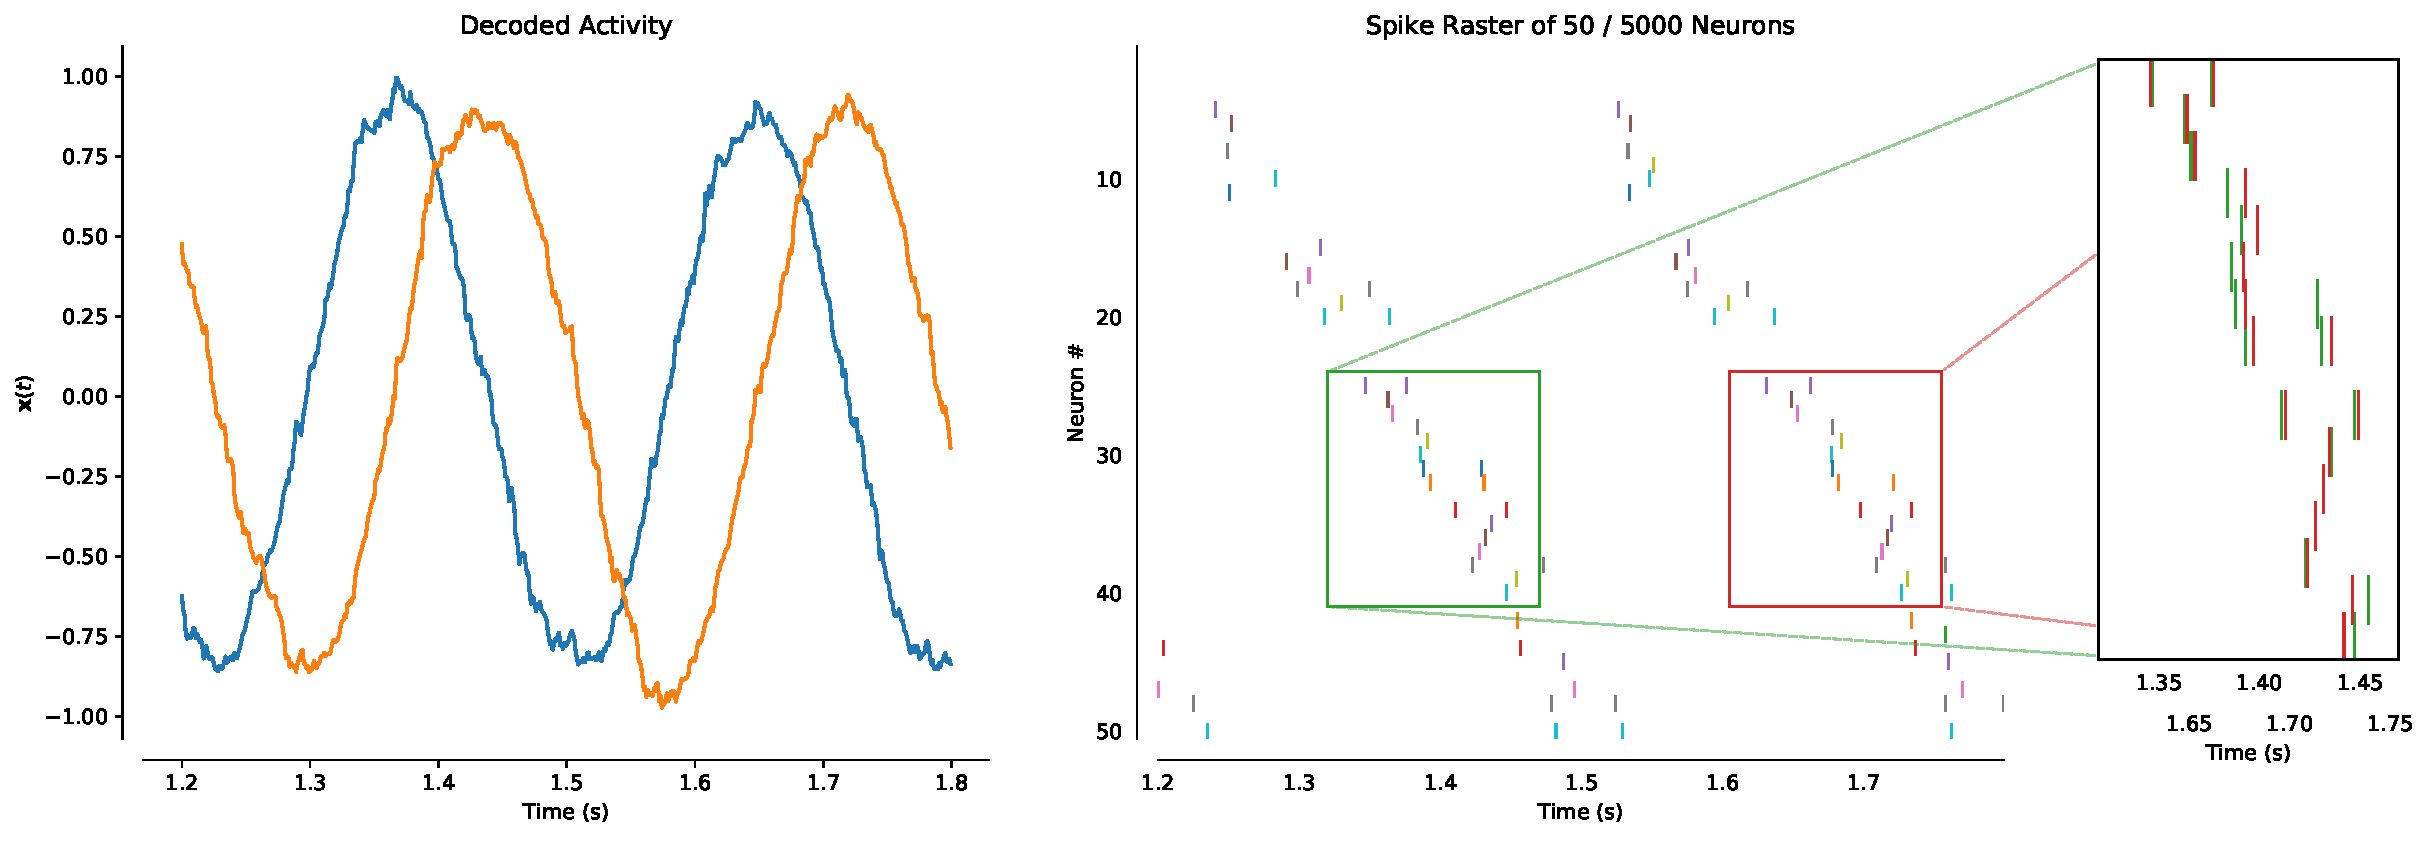
\includegraphics[width=\textwidth]{spike-time-coding}
     
    \caption{\label{fig:spike-time-coding} 
      Demonstrating the semantic ambiguity between ``spike-time coding'' and ``rate-coding'' in the context of a standard NEF-optimized network.
      (Left)~An ensemble of \numprint{5000} LIF neurons with random 2D encoders and uniform $[0.5, 1]$ intercepts are trained to oscillate at approximately $3.5$\,Hz.
      We omit the first $1.2$ seconds of simulation to wash away initial transients.
      (Right)~Spike rasters of \numprint{50} randomly selected neurons, ordered by the angle of each neuron's respective encoding vector.
      Each neuron spikes only $0$, $1$, or $2$ times per oscillation, and at a precise moment in time---on the order of milliseconds (see inset)---before remaining silent for another several hundred milliseconds.
      Thus, the precise spike-timing of each individual neuron reliably conveys information about the 2D state-space of the oscillation, despite not explicitly incorporating such a requirement into the training procedure.
      The NEF's ``post-synaptic current coding'' explains how this works (see text for details).
    }
\end{figure}

\subsection{Low-Frequency Representations}

The idea that the most amount of ``information'' is present within the low-frequency range of the signals, relative to the firing rates of neurons and time-constants of synapses.

Maybe additional biological detail can get around this limitation, or maybe the time-constants are this way for this very reason.


\section{Suitability for Neuromorphic Hardware}

\citep{boahen2017neuromorph}

\subsection{Optimality of Spike Coding}
\label{sec:spike-coding}

\begin{figure}
  \centering
  \begin{subfigure}{\textwidth}
    \centering
    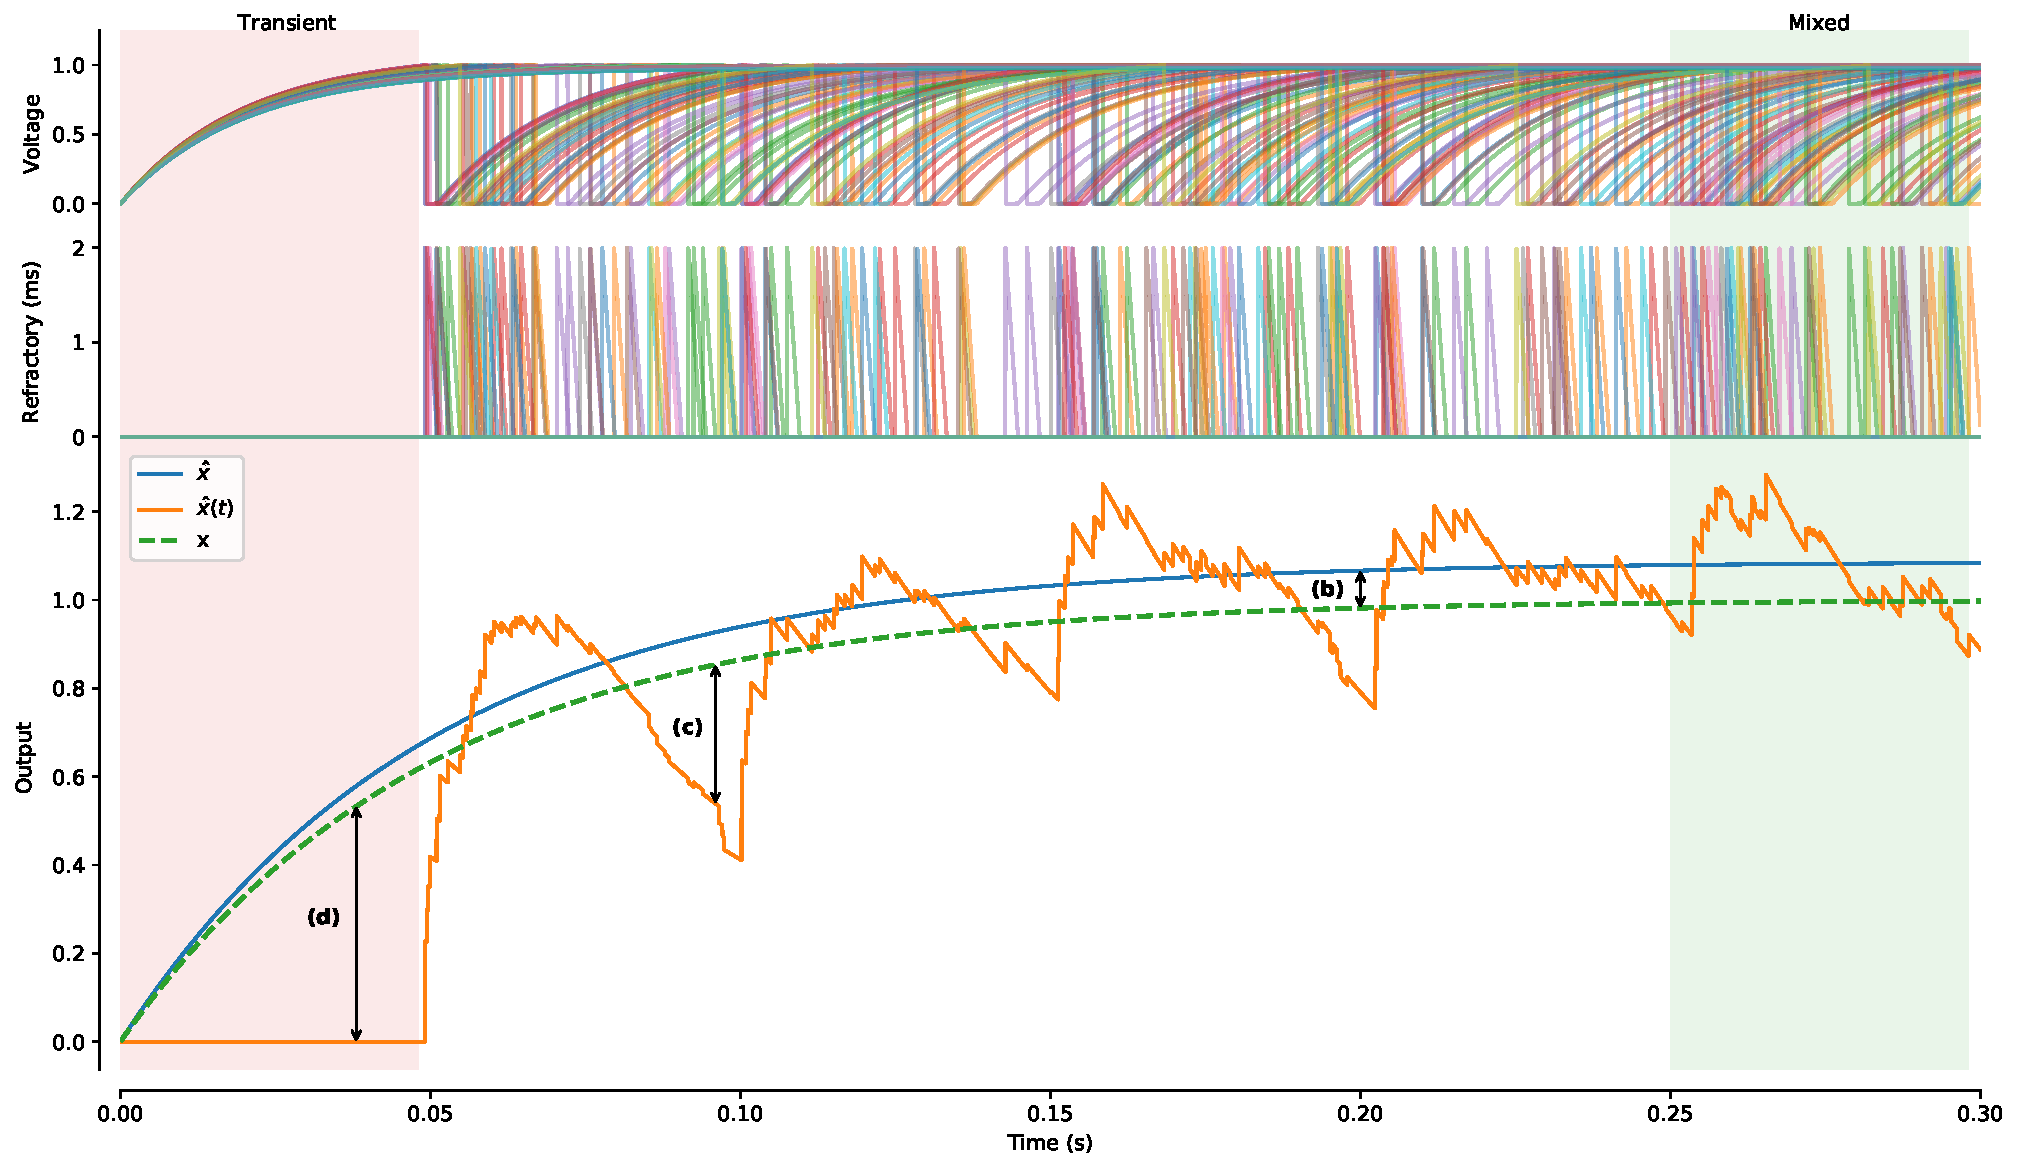
\includegraphics[width=\linewidth]{nef-error-types-a}
    \caption{Example Network Simulation}
    \label{fig:nef-error-types-a}
  \end{subfigure}
  \begin{subfigure}{.33\textwidth}
    \centering
    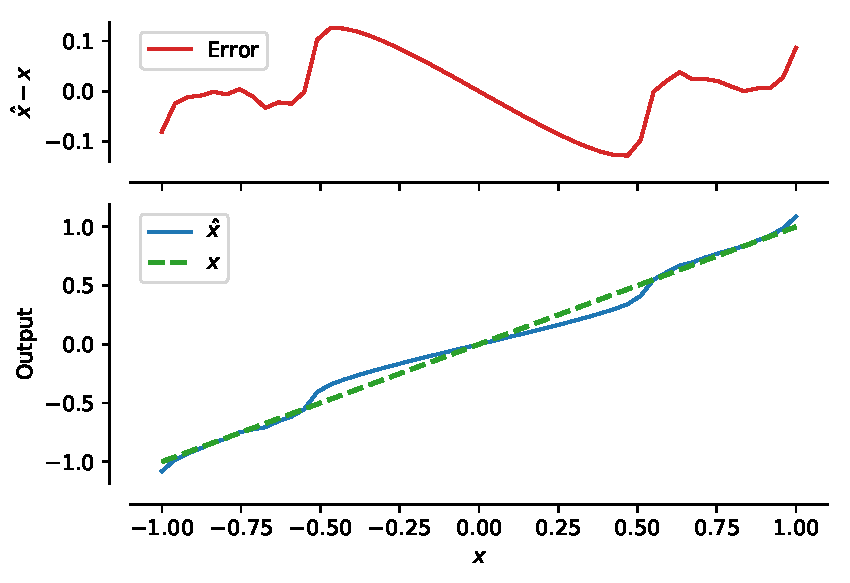
\includegraphics[width=\linewidth]{nef-error-types-b}
    \caption{Static Distortion}
    \label{fig:nef-error-types-b}
  \end{subfigure}%
  \begin{subfigure}{.33\textwidth}
    \centering
    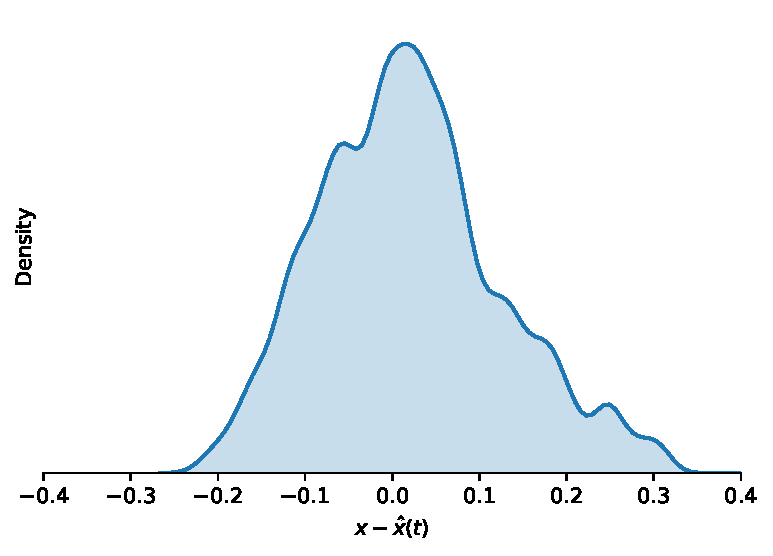
\includegraphics[width=\linewidth]{nef-error-types-c}
    \caption{Spiking Noise}
    \label{fig:nef-error-types-c}
  \end{subfigure}%
  \begin{subfigure}{.33\textwidth}
    \centering
    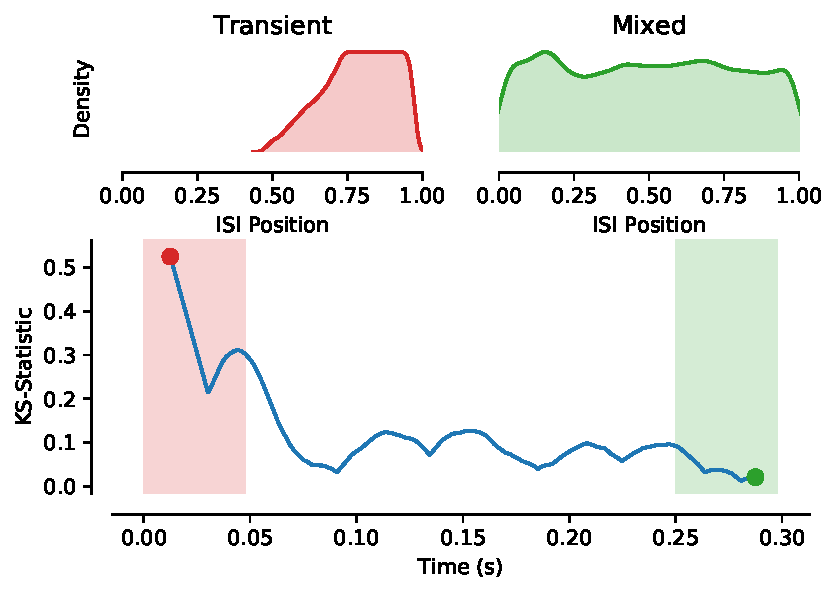
\includegraphics[width=\linewidth]{nef-error-types-d}
    \caption{State-Discrepancy}
    \label{fig:nef-error-types-d}
  \end{subfigure}
  \caption{ \label{fig:nef-error-types}
    Summarizing the three types of error in a standard NEF network.
(c) Noise KS-Test: KstestResult(statistic=0.06581452914138136, pvalue=1.1330796855568144e-75)
(d) Maximum p-value: 6.984832323950607e-16
  }
\end{figure}

Mention the spike-time decoder optimization (Temporal Solver) for more detailed neurons.

Also Appendix from NEF text on synaptic versus somatic dynamics.

\subsubsection{Integrating a Spiking LIF Neuron}

We feed a constant input to a population of neurons, initially at rest, such that the the $i^{th}$ neuron spikes at a rate of $a_i$ hertz. The synapse is an integrator that will simply count spikes and output the count divided by the elapsed time $t$. This gives a one-sided estimate of the true spike rate, that is essentially equivalent to using a lowpass with infinite $\tau$.

Let $\V{\tilde{x}}(t)$ be the estimate obtained by decoding the above using the usual decoders $\V{d}$. Now observe that since $\floor{a_i t}$ is the number of times the $i^{th}$ neuron has spiked after $t$ seconds, we get:
\begin{align*}
\V{\tilde{x}}(t) &= \sum_i \V{d}_i \floor{a_i t} / t .
\end{align*}

\begin{align*}
\implies \quad \V{\hat{x}} - \V{\tilde{x}}(t) &= \sum_i \V{d}_i (a_i - \floor{a_i t} / t) \\
&= \sum_i \V{d}_i \frac{a_i t - \floor{a_i t}}{t} \\
&= \frac{1}{t} \sum_i \V{d}_i \Delta_i(t)
\end{align*}
where
\begin{align*}
\Delta_i(t) := a_i t - \floor{a_i t}, \quad 0 \le \Delta_i(t) < 1
\end{align*}
is the ``truncation'' error, obtained by rounding down to the start of the inter-spike interval at time $t$.
\begin{align*}
\implies \quad 0 \le \V{\hat{x}} - \V{\tilde{x}}(t) < \frac{1}{t} \sum_i \V{d}_i .
\end{align*}

This reveals that the error is bounded above by $O(t^{-1})$.

As an aside, since decoders grow inversely with firing rate, using neurons with higher firing rates will improve the error, as you would expect. However it is slightly counter-intuitive that adding more neurons won't increase the worst-case accuracy\footnote{The sum of all decoders is invariant to $n$.}. But observe that the worst-case is only obtained if all of the neurons collude to force $\Delta_i(t) \approx 1$ simultaneously. We will see later that less pessimistic bounds can be obtained probabilistically by assuming $\Delta_i(t)$ is sampled independently from a reasonable distribution (and then the number of neurons will matter). 

\subsubsection{Lowpass Filtering a Spiking LIF Neuron}

Suppose we feed a constant input to the $i^{th}$ neuron, which then spikes at a rate of $a_i > 0$ hertz, with the first spike occurring at some time $0 \le s_i < 1/a_i$. Filter each spike with a lowpass $h(t) = (1 / \tau) e^{-t/\tau}$. Suppose for now that the synapse is initially at rest, but this will be easy to account for at the end by linearity. % (simply add the initial state times $e^{-t/\tau}$).

Let $\tilde{a}_i(t; s_i)$ be the estimated firing rate at time $t$ given that the first spike occurs at $s_i$. By translating the above description,
\begin{align*}
\tilde{a}_i(t; s_i) &= \sum_{0 \le j \le a_i(t - s_i)} (\delta_{j / a_i + s_i} \ast h)(t) \\
&= \sum_{0 \le j \le a_i(t - s_i)} \frac{1}{\tau} e^{-(t - (j/a_i + s_i))/\tau} \\
&= \sum_{0 \le j \le a_i(t - s_i)} \frac{1}{\tau} (\underbrace{e^{-1/a_i \tau}}_{r_i})^{a_i(t - s_i) -j} 
\end{align*}
where $0 < r_i < 1$ is an important quantity that we remark is invariant to time, and depends only on the firing rate and $\tau$.
\begin{align}
\label{eq:neuron}
\implies \quad \tilde{a}_i(t; s_i) &= \frac{r_i^{a_i(t - s_i) + 1}}{\tau} \sum_{1 \le j \le a_i(t - s_i) + 1} \left( r_i^{-1} \right)^j, \quad \text{(note: change of index)} \nonumber \\
&= \frac{r_i^{a_i(t - s_i) + 1}}{\tau} \left( \frac{1}{r_i} \right) \frac{\left( \frac{1}{r_i} \right)^{\floor{a_i(t - s_i) + 1}} - 1}{\frac{1}{r_i} - 1}, \quad \text{by the geometric series} \nonumber \\
\Aboxed{ &\,= \frac{r_i^{\Delta_i(t; s_i)} - r_i^{a_i(t - s_i) + 1}}{\tau(1 - r_i)}}
\end{align}
where
\begin{equation}
\begin{gathered}
\label{eq:delta}
\Delta_i(t; s_i) := (a_i(t - s_i) + 1) - \floor{a_i(t - s_i) + 1} = a_i(t - s_i) - \floor{a_i(t - s_i)} \\
0 \le \Delta_i(t; s_i) < 1 .
\end{gathered}
\end{equation}
is again the same truncation error, but shifted to account for $s_i$. It is helpful to think of this geometrically: $\Delta_i(t; s_i)$ is simply the unit line rotated by $a_i s_i$ (modulo $1$).

\begin{figure}[h!]
\centering
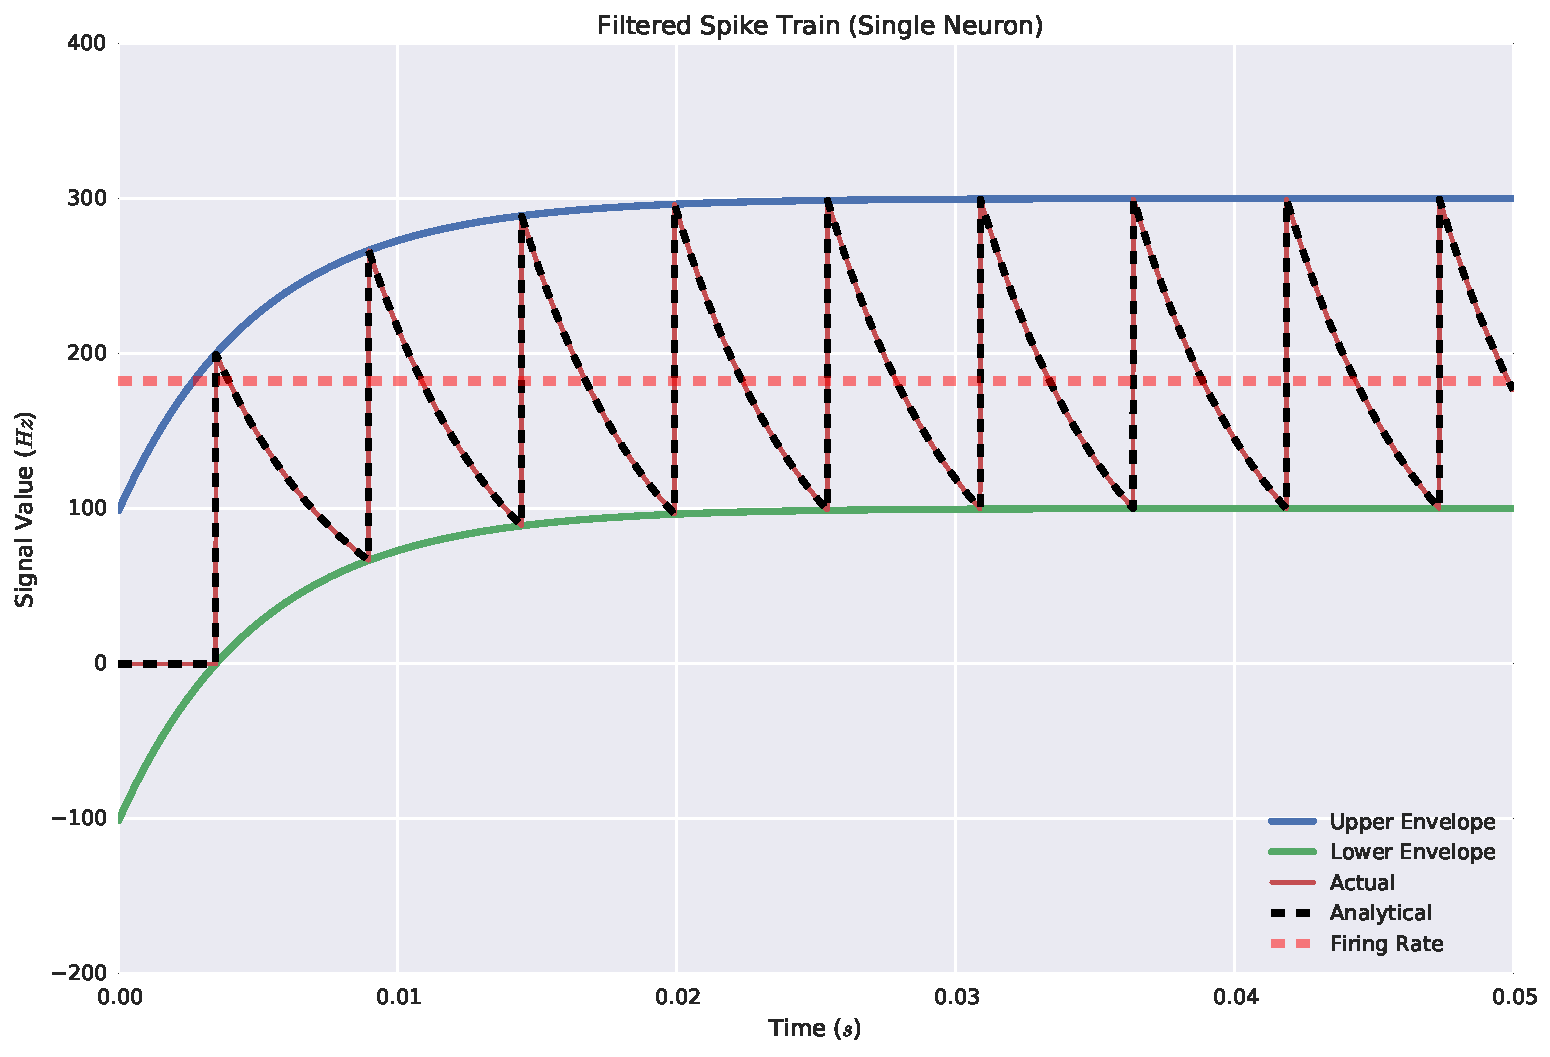
\includegraphics[width=1.0\textwidth]{slif-filtered}
\caption{\label{fig:slif-filtered} Filtered spike train under constant input ($\tau = 5\,$ms), matched by equation (\ref{eq:neuron}) and its bounds.}
\end{figure}

The boxed equation (\ref{eq:neuron}) perfectly characterizes the neuron's filtered spike train under the given assumptions. In addition, the lower/upper bounds of $\Delta_i(t; s_i)$ give the upper- and lower-envelopes, respectively:
\begin{equation*}
\frac{r_i - r_i^{a_i(t - s_i) + 1}}{\tau(1 - r_i)} < \tilde{a}_i(t; s_i) \le \frac{1 - r_i^{a_i(t - s_i) + 1}}{\tau(1 - r_i)} .
\end{equation*}

We also remark that for the LIF case, $s_i$ can be easily determined from the neuron's initial state and its input current $J_i$:
\begin{align*}
v_i(t) &= v_i(0) + (J_i - v_i(0))(1 - e^{-t/\tau_{RC}}) \\
\implies \quad s_i &= -\tau_{RC} \ln \frac{J_i - 1}{J_i}
\end{align*}
where $\tau_{RC}$ is the neuron's membrane time-constant. See \href{https://github.com/nengo/nengo/pull/975}{PR \#975} for details.

The analysis from \S\ref{sec:lowpass} can be used to obtain the precise form of the decoded estimate $\V{\tilde{x}}(t)$ at the population level. However, this depends on the initial spikes $s_i$, and so $\V{\tilde{x}}(t)$ can vary wildly depending on the initial state of all neurons.

For instance, if all neurons are initially at rest, then the estimate is most certainly zero until the fastest neuron fires. More critically, if all neurons have the same firing rate, but their initial spikes are not evenly distributed, then the error at the population level will be the addition of all their envelopes (as in the aside from the end of \S\ref{sec:integrator}).

For this work, we essentially assume that we have no control over the initial state of the system. That is, we suppose that the state of each neuron at $t = 0$ is independent and ``random'' (i.e., the previous input could have switched at any time). To be precise, we interpret $s_i$ as the realization of a random variable $S_i$ distributed by some chosen probability distribution.

Although the following analysis lends itself to the use of arbitrary distributions, some preliminary experimentation has shown that it is reasonable to assume:
\begin{equation}
\begin{gathered}
\label{eq:s}
S_i \sim U[0, 1/a_i] \\
\implies \quad f_{S_i}(s_i) = a_i \quad .  \quad \quad 
\end{gathered}
\end{equation}

This implies that the neuron is not initially biased to spike at any time in particular. In order for this to occur, we essentially require that the majority of neurons had non-zero activity in response to their prior input. In that situation, an arbitrary neuron could be at any point along its inter-spike interval, since it is not colluding with any other neurons.

In the NEF, this is typically a fair assumption, given that the tuning curves are broad (non-zero for half of the input space on average), and spike trains tend to be independent. However, for sparser encodings, or relatively large changes in input, the distribution becomes skewed towards $1 / a_i$. Similarly, if firing tends to be nearly synchronous, then the neurons will over-estimate whenever they spike together. This is noteworthy because this theory may give quantitative predictions regarding these trade-offs between encoding sparsity and firing rates, versus the desired accuracy and latency (see discussion).

Now, the analysis proceeds as follows. Fix $t$\footnote{This can be interpreted as the time that we decide to observe/measure the state of the system.} and then independently sample each $s_i$. This determines $\Delta_i(t; s_i)$ for each neuron, by the cyclic rotation $a_i s_i$ (modulo $1$) from (\ref{eq:delta}). We then define the random variable $\tilde{A}_i(t) := \tilde{a}_i(t; S_i)$, which we should understand as being distributed by ``mapping'' $S_i$ through the function $\tilde{a}_i$ for some chosen $t$. As an aside, for the special case of uniform $S_i$, the mapping $\tilde{a}_i$ actually corresponds to a cyclically shifted version of the inverse CDF of $\tilde{A}_i(t)$\footnote{This requires a subtle monotonicity argument. The CDF of $\tilde{A}_i$ can therefore be derived by inverting the unshifted $\tilde{a}_i$, but the result is not very nice to work with due to some discontinuities in its derivative.}.
%\begin{align}
%\label{eq:z}
%z_i(s_i; t) := \tilde{a}_i(t; s_i)
%\end{align}
%to view $Z_i(t)$ as a random variable that is obtained by ``mapping'' the distribution of $S_i$ through the function $\tilde{a}_i$ for some chosen $t$.  

Then the random variable $\V{\tilde{X}}(t) := \sum_i \V{d}_i \tilde{A}_i(t)$ is the decoded estimate obtained by forming a mixture of $\tilde{A}_i(t)$. The following subsections will analyze the expectation and variance of each $\tilde{A}_i(t)$ to determine the expected error and variability at time $t$.

\subsubsection{Expected Error}

By the law of the unconscious statistician (LOTUS) applied to $\tilde{A}_i(t)$:
\begin{align}
\label{eq:a_expectation}
E \left[ \tilde{A}_i(t) \right] &= \int_D \tilde{a}_i(t; s_i) f_{S_i}(s_i) \,ds_i, \quad \text{where $D$ is the domain of $S_i$} \nonumber\\
          &= \int_D \frac{r_i^{\Delta_i(t; s_i)} - r_i^{a_i(t - s_i) + 1}}{\tau(1 - r_i)} f_{S_i}(s_i) \,ds_i, \quad \text{by (\ref{eq:neuron})} \nonumber\\
          &= \frac{1}{\tau(1 - r_i)} \left( \int_0^{1} r_i^{\Delta_i(t; s_i)} \,d\Delta_i(t; s_i) - \int_0^{1/a_i} r_i^{a_i(t - s_i) + 1} (a_i) \,ds_i \right) \nonumber\\
          &= \frac{1}{\tau(1 - r_i)} \left( (-a_i \tau) e^{-\Delta_i(t; s_i)/a_i \tau} \bigg|_{\Delta_i(t; s_i) = 0}^{1} - (a_i \tau) r_i^{a_i(t - s_i) + 1} \bigg|_{s_i = 0}^{1/a_i} \right) \nonumber\\
          &= \frac{a_i}{(1 - r_i)} \left(  (1 - r_i) - (r_i^{a_i t} - r_i^{a_i t + 1})  \right) \nonumber\\
          &= a_i (1 - e^{-t/\tau}) .
\end{align}

Including the initial state of the synapse, $\V{x}_0$, the expected error at time $t$ is:
\begin{align}
\label{eq:expectation}
\implies \quad E\left[ \V{\hat{x}} - (\V{\tilde{X}}(t) + \V{x}_0 \, e^{-t/\tau}) \right] &= \sum_i \V{d}_i (a_i - E \left[ \tilde{A}_i(t) \right]) - \V{x}_0 \, e^{-t/\tau} \nonumber \\
&= \sum_i \V{d}_i a_i e^{-t/\tau} - \V{x}_0 \, e^{-t/\tau} \nonumber  \\
\Aboxed{ &\,= (\V{\hat{x}} - \V{x}_0) e^{-t/\tau} . }
\end{align}

\begin{figure}[h!]
\centering
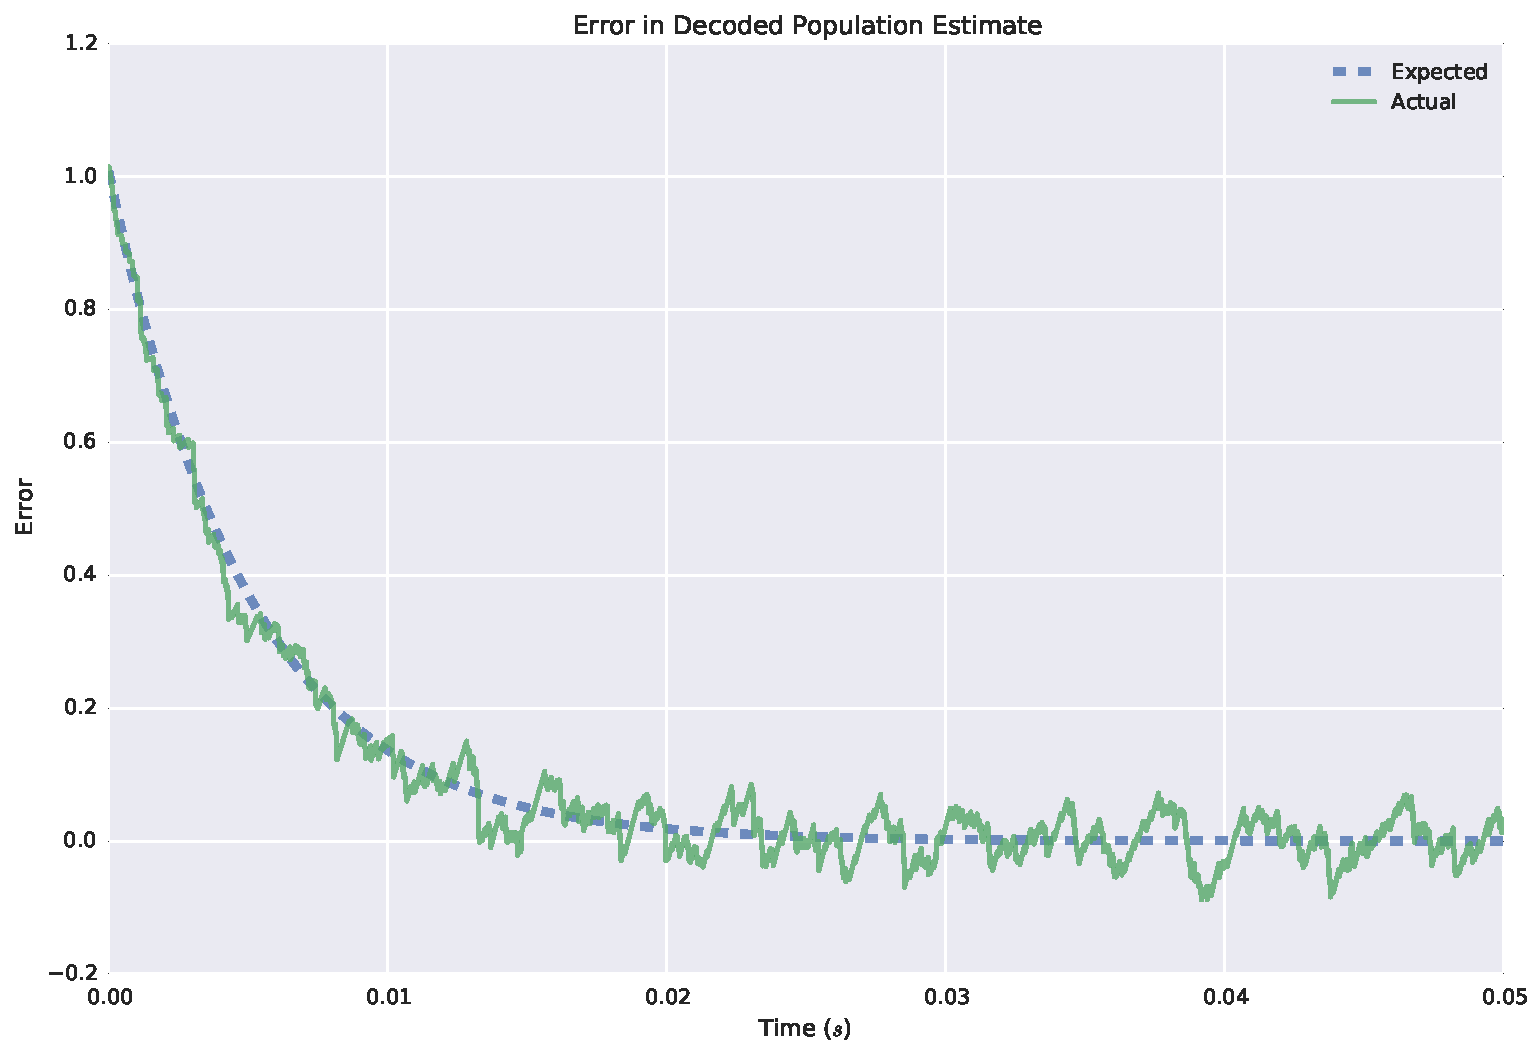
\includegraphics[width=1.0\textwidth]{slif-error}
\caption{\label{fig:slif-error} Error from filtered and decoded estimate using a population of $100$ neurons ($\tau = 5$\,ms, $\V{x}_0 = -0.2$, and $\V{\hat{x}} \approx \V{x}_0 + 1$). The expectation from (\ref{eq:expectation}) is given by the dashed line.}
\end{figure}

On one hand this is what we should intuitively expect, since we are essentially filtering an error signal using the same lowpass with an initial state given by the initial error. But it should also be surprising that this result holds independently of the width ($1 / a_i$) of each inter-spike interval, while we have only assumed the initial spikes are uniformly distributed across these intervals (in fact the independence assumption has not been used). If all neurons were initially at rest, then this result clearly no longer holds (consider $0 < t < \min_i 1/a_i$).

This assures us that we can set $\tau \rightarrow 0$ to minimize latency without hurting the expected error. However, as we will soon see, this comes at the cost of increasing the variability of the estimate.

\subsubsection{Variance in Error}

To compute $Var \left[ \tilde{A}_i(t) \right] = E \left[ \tilde{A}_i(t)^2 \right] - E \left[ \tilde{A}_i(t) \right]^2$ we rewrite the second moment:
\begin{align*}
E \left[ \tilde{A}_i(t)^2 \right] &= E \left[ \left( \frac{r_i^{\Delta_i(t; S_i)} - r_i^{a_i(t - S_i) + 1}}{\tau(1 - r_i)} \right)^2 \right] \\
&= \left( \frac{1}{\tau(1 - r_i)} \right)^2 \left( E \left[ (r_i^{\Delta_i(t; S_i)})^2 \right ] - 2 E \left[ r_i^{\Delta_i(t; S_i) + a_i(t - S_i) + 1} \right] + E \left[ (r_i^{a_i(t - S_i) + 1})^2 \right] \right)
\end{align*}
and then separately determine each expectation.

The PDFs of $r_i^{\Delta_i(t; S_i)}$ and $r_i^{a_i(t - S_i) + 1}$ are both $a_i \tau / x$ over their respective domains. This can be seen directly:
\begin{align*}
\frac{\partial}{\partial x} Pr \left[ r_i^{\Delta_i(t; S_i)} \le x \right] &= \frac{\partial}{\partial x} Pr \left[ \Delta_i(t; S_i) \le -a_i \tau \ln x \right] \\
&= \frac{\partial}{\partial x} (1 - (-a_i \tau \ln x)) \\
&= a_i \tau / x .
\end{align*}
and the proof for $r_i^{a_i(t - S_i) + 1}$ is analogous. We remark that these two facts can be used to give a slightly different derivation for (\ref{eq:a_expectation}). 

Applying LOTUS to each of these random variables gives:
\begin{align*}
E \left[ (r_i^{\Delta_i(t; S_i)})^2 \right ] &= \int_{r_i}^1 \frac{a_i \tau}{x} x^2 \,dx = \frac{a_i \tau x^2}{2} \bigg|_{x = r_i}^1 = \frac{a_i \tau (1 - r_i^2)}{2} \\
E \left[ (r_i^{a_i(t - S_i) + 1})^2 \right] &= \int_{r_i^{a_i t + 1}}^{r_i^{a_i t}} \frac{a_i \tau}{x} x^2 \,dx = \frac{a_i \tau x^2}{2} \bigg|_{x = r_i^{a_i t + 1}}^{r_i^{a_i t}} = \frac{a_i \tau (1 - r_i^2) r_i^{2 a_i t}}{2} .
\end{align*}

To compute the remaining expectation, we need to get some further understanding of $\Delta_i(t; S_i) = (a_i(t - s_i) + 1) - \floor{a_i(t - s_i) + 1}$. Define $K_i(t) := \floor{a_i t}$ as the current interval independent of $s_i$. %Then the $i^{th}$ neuron has spiked $K_i(t - s_i) + 1 = \floor{a_i(t - s_i) + 1}$ times at time $t$. More importantly, 
The point \mbox{$s_i = t - K_i(t)/a_i \equiv t \ (\text{mod}\ 1/a_i)$} gives the discontinuity in $\Delta_i(t; s_i)$ with respect to $s_i$, because that is when the spike becomes aligned with $t$ in the current interval. Namely, if $0 \le s_i \le t - K_i(t)/a_i$, then $\floor{a_i(t - s_i) + 1} = \floor{K_i(t) + 1} = K_i(t) + 1$. Likewise, if $t - K_i(t)/a_i < s_i \le 1/a_i$, then $\floor{a_i(t - s_i) + 1} = K_i(t)$\footnote{If this is confusing, recall that we are fixing $t$ and then sweeping $s_i$ from $0$ to $1 / a_i$.}. Then use LOTUS once more, along with the above fact to split up the integral.
\begin{align*}
E \left[ r_i^{\Delta_i(t; S_i) + a_i(t - S_i) + 1} \right] &= \int_0^{1/a_i} r_i^{2(a_i(t - s_i) + 1) - \floor{a_i(t - s_i) + 1}} (a_i) \, ds_i \\
&= a_i \left( \int_0^{t - K_i(t)/a_i} r_i ^ {(2a_i t - K_i(t) + 1) - (2a_i s_i)} \, ds_i + \int_{t - K_i(t)/a_i}^{1/a_i} r_i^{(2a_i t - K_i(t) + 2) - (2a_i s_i)} \, ds_i \right) \\
&= a_i r_i^{2a_i t - K_i(t) + 1} \tau / 2 \left( e^{2s_i / \tau} \bigg|_{s_i=0}^{t - K_i(t)/a_i} + r_i e^{2s_i / \tau} \bigg|_{s_i=t - K_i(t)/a_i}^{1/a_i} \right) \\
&= a_i r_i^{2a_i t - K_i(t) + 1} \tau / 2 \left( r_i^{-2 a_i(t - K_i(t)/a_i)} - 1 + r_i^{-1} - r_i^{-2a_i(t - K_i(t)/a_i) + 1} \right) \\
&= a_i \tau (1 - r_i)(r^{K_i(t) + 1} + r_i^{2a_i t - K_i(t)}) / 2
\end{align*}

Plugging these all in then gives:
\begin{align*}
Var \left[ \tilde{A}_i(t) \right] = \, \Aboxed{ a_i \left( \frac{(1 - r_i^2)(1 + r_i^{2a_i t})}{2\tau(1 - r_i)^2} - \frac{\left( r_i^{K_i(t) + 1} + r_i^{2a_i t - K_i(t)} \right)}{\tau(1 - r_i)} - a_i(1 - r_i^{a_i t})^2 \right) }
\end{align*}

\begin{align}
\label{eq:variance}
\implies \quad Var\left[ \V{\hat{x}} - (\V{\tilde{X}}(t) + \V{x}_0 \, e^{-t/\tau}) \right] = Var\left[ \V{\tilde{X}}(t) \right]
= \sum_i \V{d}_i^2 \, Var\left[ \tilde{A}_i(t) \right] .
\end{align}

\begin{figure}[h!]
\centering
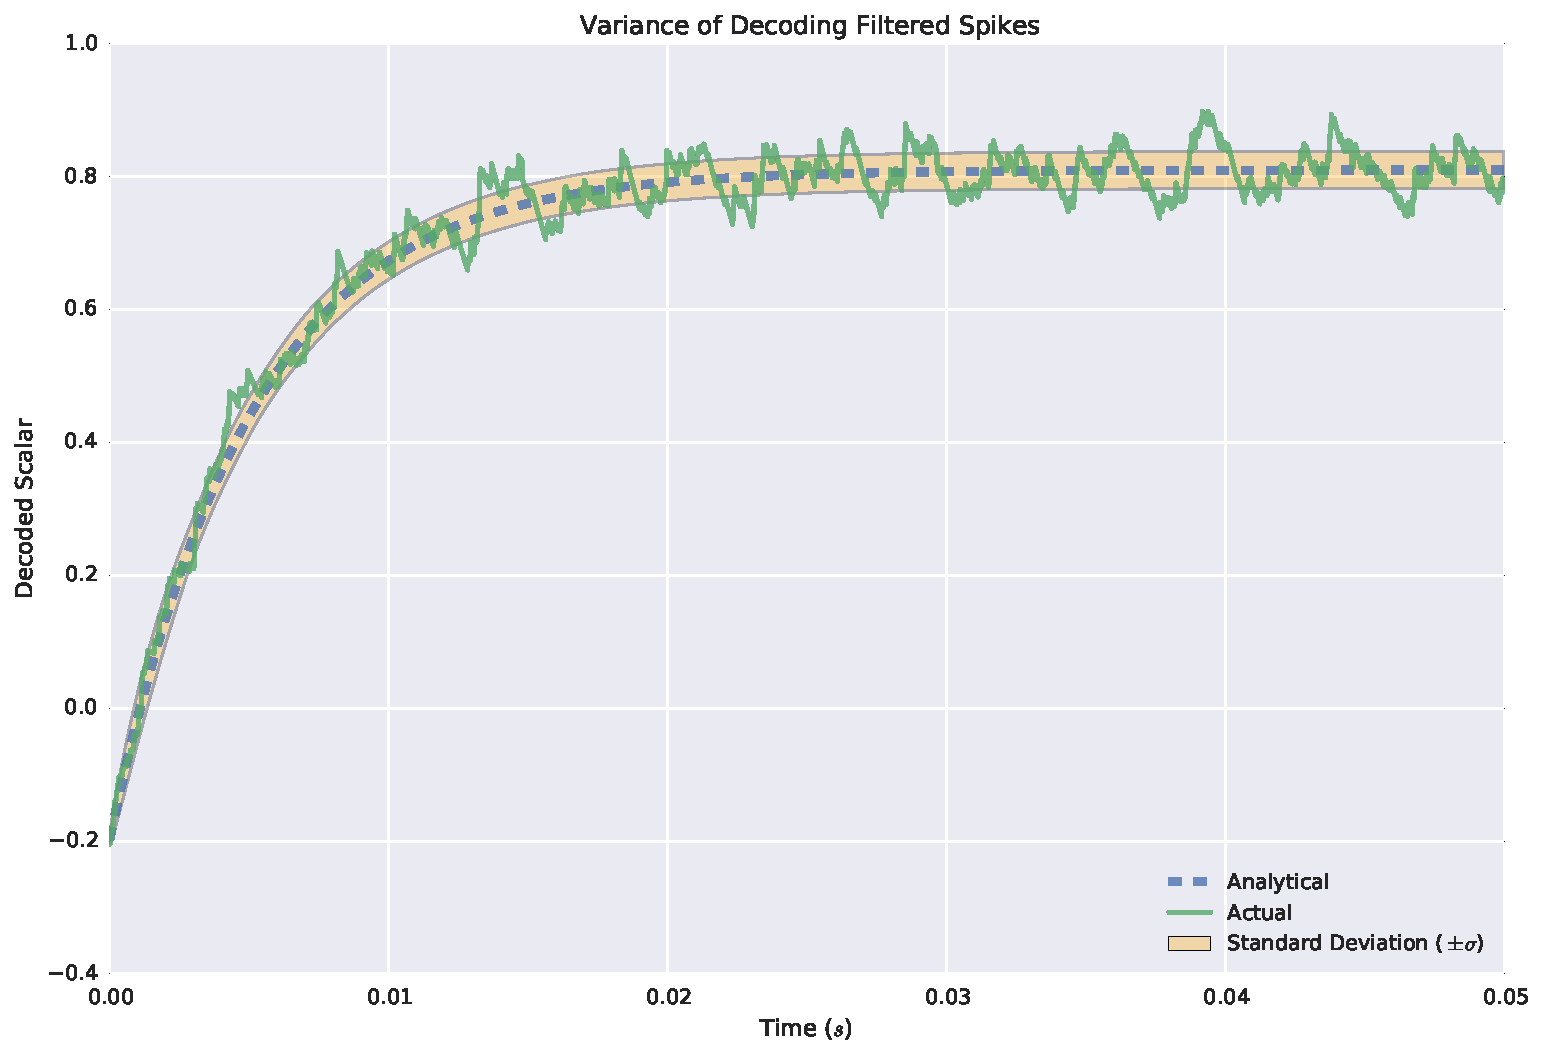
\includegraphics[width=1.0\textwidth]{slif-variance}
\caption{\label{fig:slif-variance} Filtered and decoded estimate using the same network as Fig.~\ref{fig:slif-error}. The variance is highlighted by one standard deviation from the mean.}
\end{figure}

\subsubsection{Validity of Uniform Assumption}

\begin{figure}[h!]
\centering
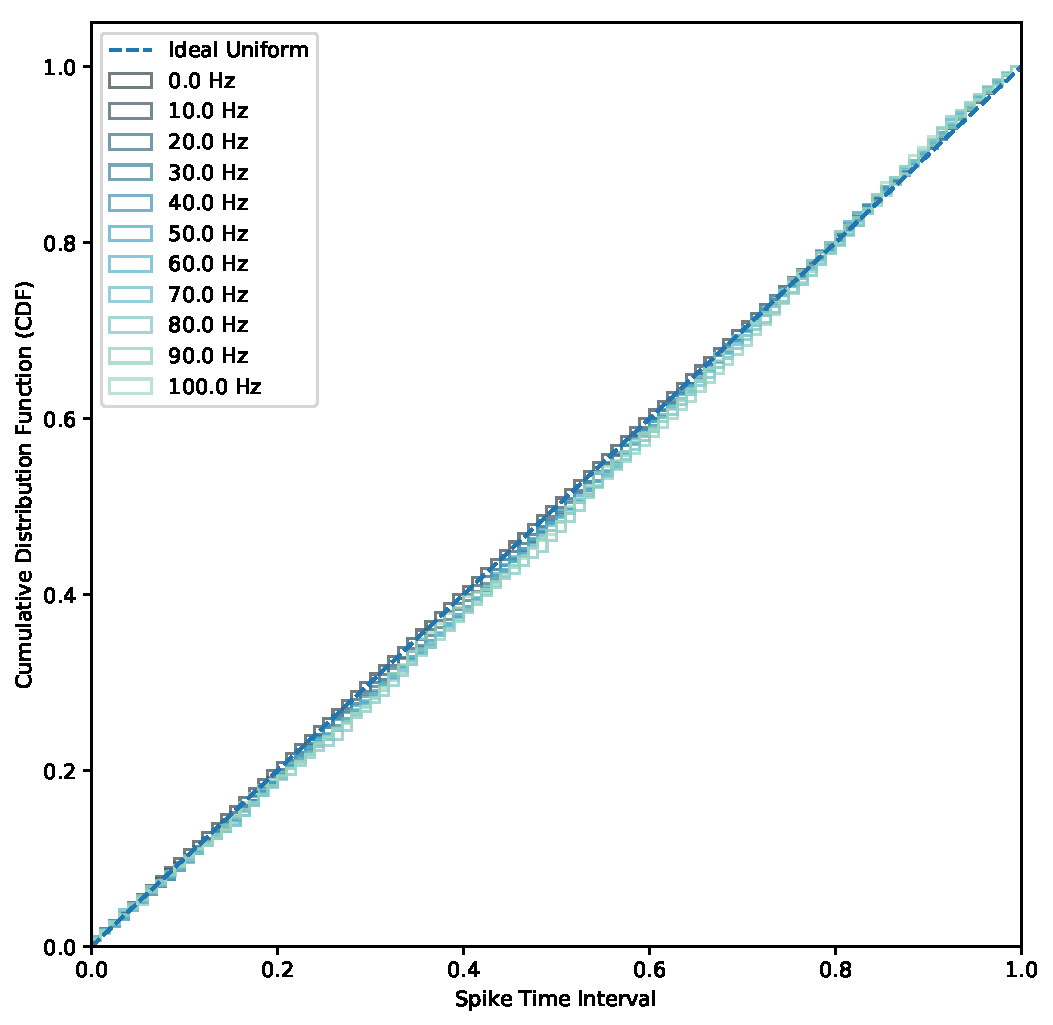
\includegraphics[width=1.0\textwidth]{spike-time-intervals}
\caption{\label{fig:spike-time-intervals} Empirical distribution of ISI positions---$s_i$ normalized by the instaneous rate $a_i$---for sinusoid stimuli of varying frequencies.
  The ideal distribution (dashed) is uniform $[0, 1]$. In the ideal case, the spiking LIF model is equal to its non-spiking counterpart in the sense of expectation.
}
\end{figure}

The previous analysis relies on the assumption that each neuron is ``uniformly ready to spike''.
To validate this assumption from equation (\ref{eq:s}) that $S_i \sim U[0, 1/a_i]$, we empirically sampled this distribution for sinusoidal test stimuli of varying frequencies (Fig.~\ref{fig:spike-time-intervals}).
We define the \emph{ISI position} as $s_i \times a_i$. This is the realization of a random variable, in the range $[0, 1]$.
Intuitively, this can be interpreted as the percent time remaining within the idealized inter-spike interval, given the current voltage of the neuron and its ideal spike rate.
A value of $0$ implies the neuron is currently spiking and $1$ implies the neuron just spiked.
This quantity is calculated by solving the LIF ODE and rearranging to obtain:
\begin{equation}
\left(\tau_\text{RC} \log\left(1 + \frac{1 - v_i}{J_i - 1}\right) + r_i \right) a_i \text{,}
\end{equation}
where $0 \le r_i \le \tau_\text{ref}$ is the time remaining in the refractory period.

As shown in Fig.~\ref{fig:spike-time-intervals}, the default LIF model ($\tau_\text{RC} = 20$\,ms, $\tau_\text{ref} = 2$\,ms, and tuning curves uniformly distributed to achieve maximum firing rates of $200-400$\,Hz) closely follows the ideal uniform distribution for input frequencies up to $100$\,Hz. For $0$\,Hz (constant) inputs, the two distributions are the same (Kolmogorov-Smirnov statistic\footnote{
The maximum absolute distance between the empirical and model CDFs.
If samples are drawn from the model distribution, its Kolmogorov-Smirnov statistic approaches $0$ with probability $1$ as the number of samples approaches infinity.}%
$<0.0002$, $p$-value~$> 1-\numprint{e-15}$).
This verifies the numerics of our spiking LIF implementation\TODO{cite Nengo LIF improvements}, as we should expect that a constant input causes each neuron to spend an equal amount of time at each position within its ideal ISI.
For changing inputs, however, the uniform assumption immediately breaks down ($p$-value~$< \numprint{e-67}$), but non-catastrophically, as the Kolmogorov-Smirnov statistic remains bounded above by $0.0335$.

Taken together, this means that any approximation error arising from the substitution of spiking LIF for non-spiking LIF models must arise from two sources: (1) the variability in equation \ref{eq:variance}, which is a function of $\tau$, the number of neurons, and the magnitude of the decoders, and (2) a systematic bias (Fig.~\ref{fig:spike-time-intervals}) resulting from the ISI positions being non-uniform with respect to the input stimuli.
In summary, this provides a theoretical framework for understanding the differences between spiking and non-spiking neuron models in the context of some desired PSC.
This also provides some theoretical justification for using spiking LIF models following an offline optimization using static tuning curves -- a procedure that the NEF and Nengo use regularly.
Lastly, this suggests criteria for optimizing the information-processing capabilities of spiking neurons in the context of high-frequency signals, as done in section~\ref{sec:poisson-spiking}.

\TODO{Comment on dimensional analysis for speeding up / slowing down timescales}

\subsection{Efficiency in Time and Space}

Low-rank factorization is optimal in space and time assuming linear weights (there is no advantage to factoring it any further by linearity).

\subsection{Turing-Completeness}


\subsection{Robustness}

Robustness to noise.

Also Conjecture: Den\`eve doesn't work in chaotic settings. NEF does (voltage vector is chaotic). NEF and FORCE are doing the same thing -- the latter just adds extra chaos in because Reservoir Computing.



Expose the general ideas about mapping NEF networks onto neuromorphic hardware, and what makes it better than other frameworks.


\subsection{Extensibility}

Section~\ref{chapt:nef-extensions}.
